\documentclass{article}
\usepackage[utf8]{inputenc}
\usepackage{amssymb}
\usepackage{graphicx}
\usepackage{setspace}
\usepackage{listings}
\usepackage{float}
\usepackage{xcolor}
\usepackage{amsmath}
\usepackage{pgfplots}
\usepackage{subcaption}
\usepackage{hyperref}

\title{\textbf{High Performance Computer Architectures Practical Course \\ - Exercise 7 -} \\[10mm]}
\author{Tutorium 1 \\[10mm] David Jordan (6260776) \\[1mm] Florian Rüffer (7454628) \\[1mm] Michael Samjatin (7485765) \\[10mm]}


\lstset{
    language=C++,
    basicstyle=\ttfamily,
    keywordstyle=\color{blue},
    stringstyle=\color{red},
    commentstyle=\color{green},
    numbers=left,
    numberstyle=\normalsize,
    breaklines=true,
    showstringspaces=false,
    frame=single,
    linewidth=1\linewidth,
    captionpos=b
}
\renewcommand{\lstlistingname}{File}% Listing -> Algorithm
\renewcommand{\lstlistlistingname}{List of \lstlistingname s}% List of Listings -> List of Algorithms

\begin{document}
\maketitle
\newpage
\section*{0\_HelloWorldParallel}
In this task we need to parallelize a HelloWorld program with OpenMP.
We start of by creating 10 threads (line 3):

\begin{lstlisting}[caption=Step 1]
    int main() {

    #pragma omp parallel num_threads(10)
    {
      int id = 0;
      
      cout << " Hello world " << id <<  endl;
    }
  
    return 0;
  }
  
}
\end{lstlisting}
This creates a more or less unexptected output, which can be traced back to the threads not being synchronized.
To solve this issue, we will synchronize our threads by adding 'omp critical' to the parallel environmnet (line 7):

\begin{lstlisting}[caption=Step 2]
    int main() {

    #pragma omp parallel num_threads(10)
    {
      int id = 0;
      
      #pragma omp critical
      {
      cout << " Hello world " << id <<  endl;
      }
    }
  
    return 0;
  }
  
\end{lstlisting}

We still need to get the id of our threads, to know which thread computed which output.
Basically which 'Hello World' is printed out by which one of the ten threads.
To do this we get the thread id like this (line 5):
\begin{lstlisting}[caption=Step 2]
    int main() {

    #pragma omp parallel num_threads(10)
    {
      int id = omp_get_thread_num();
      
      #pragma omp critical
      {
      cout << " Hello world " << id <<  endl;
      }
    }
  
    return 0;
  }
\end{lstlisting}
At this point we can compare what happens, if we forget to properly synchronize our threads.
\begin{figure}[H]
    \centering
    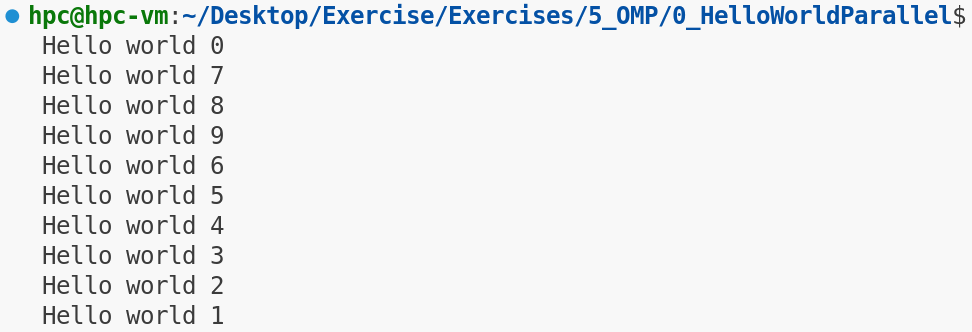
\includegraphics[scale=0.6]{no-critical.png} 
    \caption{w/o synchronization}
    \label{fig:graph}
\end{figure}
\begin{figure}[H]
    \centering
    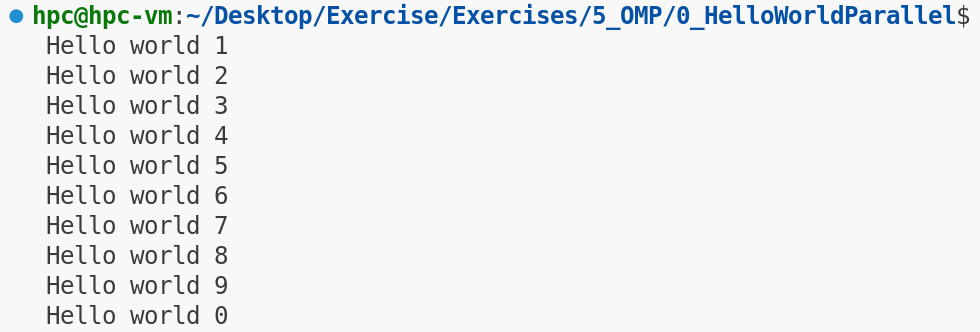
\includegraphics[scale=0.6]{with-critical.png} 
    \caption{w/ synchronization}
    \label{fig:graph}
\end{figure}
We can see that the id's are completely out of order, if the leave the synchronization out.
By adding it the output is perfectly in order.
\section*{1\_Bugs}
In this task we will examine four bugs and how to fix them.
\subsection*{Bug1}
If we run this code, we receive an error telling us, that the output array we tried to copy is not correct.
This can be fixed by editing the following lines of code:
\begin{lstlisting}[caption=Step 2]
  #pragma omp parallel firstprivate(N) num_threads(NThreads)
  {
      #pragma omp for 
      for(int i=0; i<N; i++)
      output[i] = input[i];
      }
\end{lstlisting}
Especially changing line 1 to firstprivate instead of just private.
This error occurs because 'private' is not initializing the values properly.
With 'private' each thread has its own local copy of the value, but it is not kept while entering or exiting the private region
and therefore also does not effect the value of the variable in the 'master thread'.
\subsection*{Bug2}
Again our output array is not correct.
Now the problem lies in the tmp variable of this code snippet:
\begin{lstlisting}[caption=Step 2]
tmp = 0;
#pragma omp parallel num_threads(NThreads)
{
  #pragma omp for 
  for(int i=1; i<N; i++)
  {
    tmp += i;
    outputParallel[i] = float(tmp)/float(i);
  }
}
\end{lstlisting}
The variable tmp will be used by multiple threads, leading to multiple threads updating the same value at the same time.
This will lead to a corrupted variable and incorrect results.
To solve this issue we need to make the calculation independent from the iteration (independent from the results of previous iterations).

\begin{lstlisting}[caption=Step 2]
    tmp = 0;
    #pragma omp parallel num_threads(NThreads)
    {
      #pragma omp for 
      for(int i=1; i<N; i++)
      {
        float tmp = (1+i)*i/2; // arithmetical progression
        outputParallel[i] = float(tmp)/float(i);
      }
    }
    \end{lstlisting}
\subsection*{Bug3}
Here the problem can be found in line 4.
By using 'nowait' lines 12 and 13 can be executed before the sum calculation (in line 8) is finished.

\begin{lstlisting}[caption=Step 2]
    sum = 0;
    #pragma omp parallel firstprivate(N) num_threads(NThreads)
    {
      #pragma omp for nowait
      for(int i=0; i<N; i++)
      {
        #pragma omp atomic
        sum += input[i];
      }
  
      #pragma omp for 
      for(int i=0; i<N; i++)
        outputParallel[i] = input[i]/sum;
    }
\end{lstlisting}
To fix this we can cut out the 'nowait' completely.
So we calculate the sum first and then continue with filling 'outputParallel'
\begin{lstlisting}[caption=Step 2]
    sum = 0;
    {
  
      for(int i=0; i<N; i++)
      {
        sum += input[i];
      }
      
      #pragma omp parallel firstprivate(N) num_threads(NThreads)
      #pragma omp for 
      for(int i=0; i<N; i++)
        outputParallel[i] = input[i]/sum;
    }
\end{lstlisting}
\subsection*{Bug4}
By using 'nowait' in the previous bug, we didn't wait for relevant code to finish calculations properly.
Now we need to add a barrier to ensure, that relevant calculations finish before other start.
\begin{lstlisting}[caption=Step 2]

    #pragma omp atomic
    sum += sumLocal;
    
    #pragma omp barrier
    
    #pragma omp for
    for(int i=0; i<N; i++)
    outputParallel[i] = input[i]/sum;
    }
\end{lstlisting}
Here we place a barrier just after the final sum calculations.
It is crucial for the sum to finish, before other calculations (which use the sum) can start.
As this is just an excerpt, we would need to add this line right after line 72 in the original code.

\section{Pi}
\subsection{omp parallel and OpenMP}
First, we need to specify the number of threads (in this case 2) and a
variable to store the sums, that are calculated by each thread. Therefore
the array has the lengt of the number of threads, initialized with the
value 0:
\begin{lstlisting}[caption=]
    const int nThreads = 2;
    double sums[nThreads] = {0};
\end{lstlisting}
Another important task is to save the id of the threads, so that they
can be addressed and saved correctly in the "cache-sum-list".
Because we split these steps into 2 threads, each thread only needs
to calculate one half \\(steps / thread\_count). On last thing to pay
attention is the calculation of x. Here we need to factor in the offset
for the current thread. Last but not least we need to calculate the sums
in the "cache-sum-list" and do the final computations.

\subsection*{Least amount of changes}
This can quickly be done by adding one line of code before the loop:
\begin{lstlisting}[caption=]
    #pragma omp parallel for reduction(+ : sum) private(i,x)
\end{lstlisting}
The variables x and i are declared as private variables for safety reasons,
so that they do not interfer with each other. In the solution sum is
declared as one value, and not a list - this is probably for better
data consistency and the correctnerss of the final result.\\
One another advantage of OpenMP is the correctness of the code even if the library
is disabled.




\section*{Matrix}
By adding the rather simple directive before the for loops beginning in line 88:
\begin{lstlisting}[caption=]
    #pragma omp parallel for num_threads(omp_get_num_procs())
\end{lstlisting}
we can parallelize the for loop. Since there do not appear to be significant dependencies the process can be parallelized, a speed up in the matrix calculation compared to the scalar version can be achieved, as seen in the following output:
\begin{figure}[H]
    \centering
    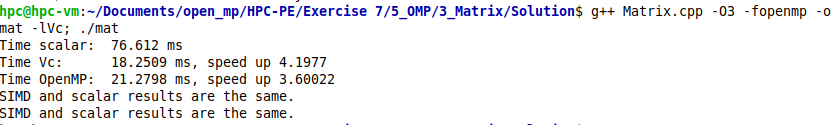
\includegraphics[scale=0.6]{matrix_output.png} 
    \caption{matrix calculation speed up}
    \label{fig:graph}
\end{figure}
However it does appear that there were some dependencies, because the Vc speed up is slightly higher with 4.1977 than OpenMP's 3.60022 speed up factor. 


\end{document}